\section{Regression Methods}
Depth estimation can be naturally formulated as a regression problem.
Every pixel $p$ of an image $\mathbf{I}$ has an associated (positive) depth value $z \in \mathbb{R}^{+}$.
Monocular depth estimation consists in regressing to that depth value pixel-wise.
The input of the developed method is an image $\mathbf{I}$ and the output a depth map $\mathbf{Z}$.

\label{sec:regression_methods}

\begin{center}
	\begin{table}
		\begin{tabular}{| c | c | c | c | c |}
			\hline
			\textbf{Year} & \textbf{Authors} & \textbf{Task} & \textbf{Loss} \\
			\hline
			2014 & Eigen et al. \cite{Eigen} & Metric DE & Scale-Invariant \\
			2015 & Eigen et al. \cite{Eigen2} & Metric DE & Scale-Invariant + reg \\
			2016 & Laina et al. \cite{Laina} & Metric DE & berHu \\
			2016 & Chen et al. \cite{DIW} & Relative DE & ranking loss \\
			\hline
		\end{tabular}
		\caption{Summary of treated pure regression methods for depth estimation. \label{table:1}}
	\end{table}
\end{center}

%%%%%%%%%%%%%%%%%%%%%%%%%%%%%%%%%%%%%%%%%
%                 EIGEN
%%%%%%%%%%%%%%%%%%%%%%%%%%%%%%%%%%%%%%%%%
\subsection{Eigen et al.}
Eigen et al. \cite{Eigen} are the first to apply deep learning to metric monocular depth estimation.
They develop a two-stage method composed of a global coarse-scale network $\mathcal{S}_{1}$ (corresponding to the "Coarse" module in figure\ref{fig:Eigen}) which predicts the overall depth map using a global view of the scene and a local fine-scale network $\mathcal{S}_{2}$ (corresponding to the "Fine" module in figure\ref{fig:Eigen}) which locally refines it.
$\mathcal{S}_{1}$ uses AlexNet \cite{AlexNet} as backbone for features encoding and decodes them using an MLP, while $\mathcal{S}_{2}$ is a shallower CNN with smaller receptive field.

% architecture 1
\begin{figure}
\centering
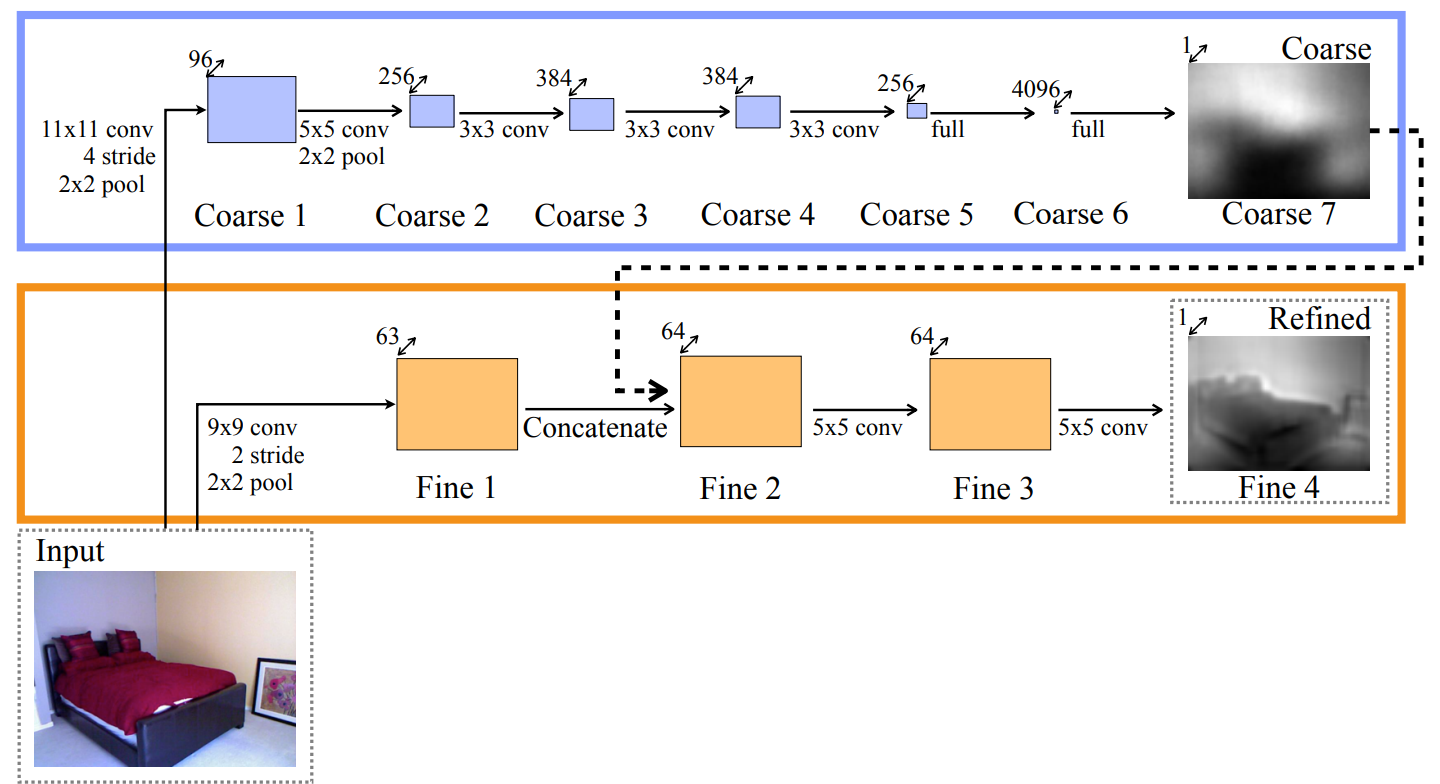
\includegraphics[width=1.\textwidth]{figs/Eigen}
\caption{Eigen et al. \cite{Eigen} two-stage architecture. \label{fig:Eigen}}
\end{figure}

% comments
The networks predict in the \textit{log-scale}, i.e. if $I$ is an input RGB image and $\mathbf{Z}$ is its depth estimate, it can be written:
\begin{equation}
	\begin{split}
	\text{log} \, \mathbf{Z}_{coarse} & = \mathcal{S}_{1}(I) \\
	\text{log} \, \mathbf{Z} & = \mathcal{S}_{2}(I, \, \text{log} \, \mathbf{Z}_{coarse})
	\end{split}
\end{equation}

% loss
Their network is trained using a scale-invariant loss function:
\[
	\delta(i, j) = \text{log} \, \mathbf{Z}^{*} (i, j) - \text{log} \, \mathbf{Z} (i, j)
\]\[
	\mathcal{L}_{scale-invariant} =
	\mathop{\text{mean}}_{(i, j) \in \mathbf{Z}^{*}} \left( \delta(i, j) \right)^{2} \quad +\quad
	\lambda \left( \mathop{\text{mean}}_{(i, j) \in \mathbf{Z}^{*}} \delta(i, j) \right) ^{2}
\]
$\lambda$ is a hyper-parameter that regulates the "scale invariace" of the loss: $\lambda$ set to $0$ reduces $\mathcal{L}_{scale-invariant}$ to a pixel-wise $l^{2}$ loss, $\lambda$ set to $1$ results in the Scale-Invariant Error exactly (introduced in "Metrics" section).
Eigen et al. opt for $\lambda = 0.5$, finding it a good compromise.
Their idea is that if a simple $l^{2}$ loss is used, then the networks probably regress to the mean depth which they proved it accounts for a large error portion.
Conversely, if a pure scale-invariant loss is used, the networks don't learn the metric structure of the scenes.

% architecture 2
\begin{figure}
\centering
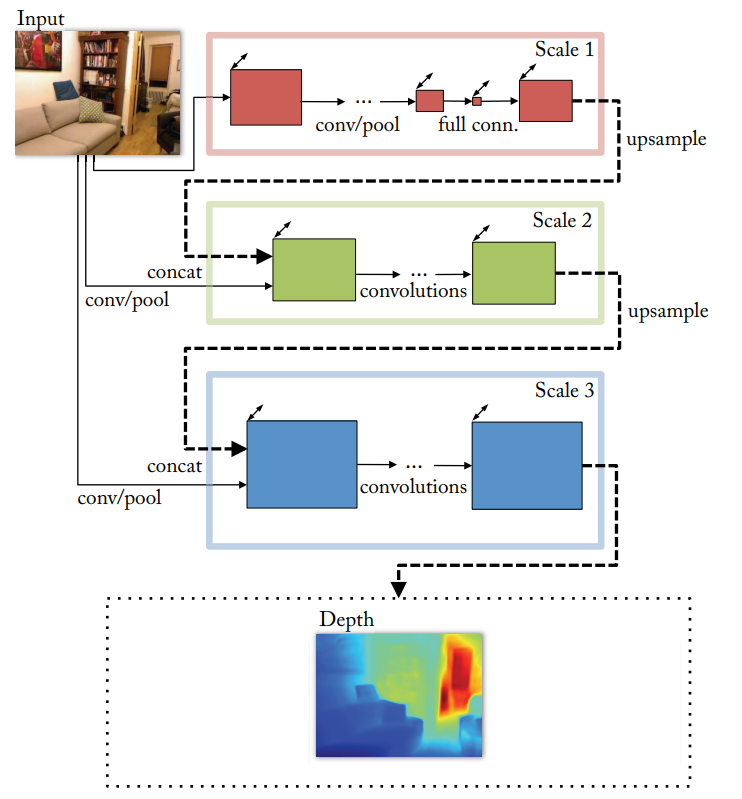
\includegraphics[scale=0.6]{figs/Eigen2}
\caption{Eigen et al. \cite{Eigen2} improved architecture, a third scale network has been added.}
\label{fig:Eigen2}
\end{figure}

% comments
Eigen et al. \cite{Eigen2} improve their previous work \cite{Eigen} by adding a third network $\mathcal{S}_{3}$ ("Scale 3" in \ref{fig:Eigen2}) working on a third finer scale and by substituting the $\mathcal{S}_{1}$ backbone with the larger VGG \cite{VGG}.
The new method has still two stages: the first composed of $\mathcal{S}_{1}$ and $\mathcal{S}_{2}$ and the second is just $\mathcal{S}_{3}$:
\[
	\text{log} \, \mathbf{Z}_{coarse} = \mathcal{S}_{2}(I, \, \mathcal{S}_{1}(I))
\]\[
	\text{log} \, \mathbf{Z} = \mathcal{S}_{3}(I, \, \text{log} \, \mathbf{Z}_{coarse})
\]

% regularization
They train their architecture using the same Scale-Invariant loss, but a regularization term is added:
\begin{equation}
\begin{split}
	\mathcal{L}_{reg} & = \mathop{\text{mean}}_{(i, j) \in \mathbf{Z}^{*}}
		\big\|
			\nabla \delta(i, j)
		\big\|_{2}^{2} \\
	& = \mathop{\text{mean}}_{(i, j) \in \mathbf{Z}^{*}}
		\big\|
			\nabla \text{log} \, \mathbf{Z}^{*} (i, j) - \nabla \text{log} \, \mathbf{Z} (i, j)
		\big\|_{2}^{2}
\end{split}
\end{equation}
This term encourages the predicted depth map to have a local structure similar to the ground-truth one by forcing predicted and ground-truth gradients to be similar (in an $l^{2}$ sense).

%%%%%%%%%%%%%%%%%%%%%%%%%%%%%%%%%%%%%%%%%
%                 LAINA
%%%%%%%%%%%%%%%%%%%%%%%%%%%%%%%%%%%%%%%%%
\subsection{Laina et al.}
Laina et al. \cite{Laina} use a fully convolutional neural network (FCNN) for regressing metric depth maps.
Their architecture is an encoder-decoder based on ResNet \cite{ResNet} and four up-sampling blocks (see figure \ref{fig:Laina}) are introduced and tested for the decoding part.
A great improvement over the work of Eigen et al. is that using an FCNN drastically reduces the number of parameters of the network, making it feasible to increase the output resolution and to work in real-time.
One difference is that Laina et al. network regresses the depth map in linear-scale and not log-scale as Eigen et al. did.

% architecture
\begin{figure}
\centering
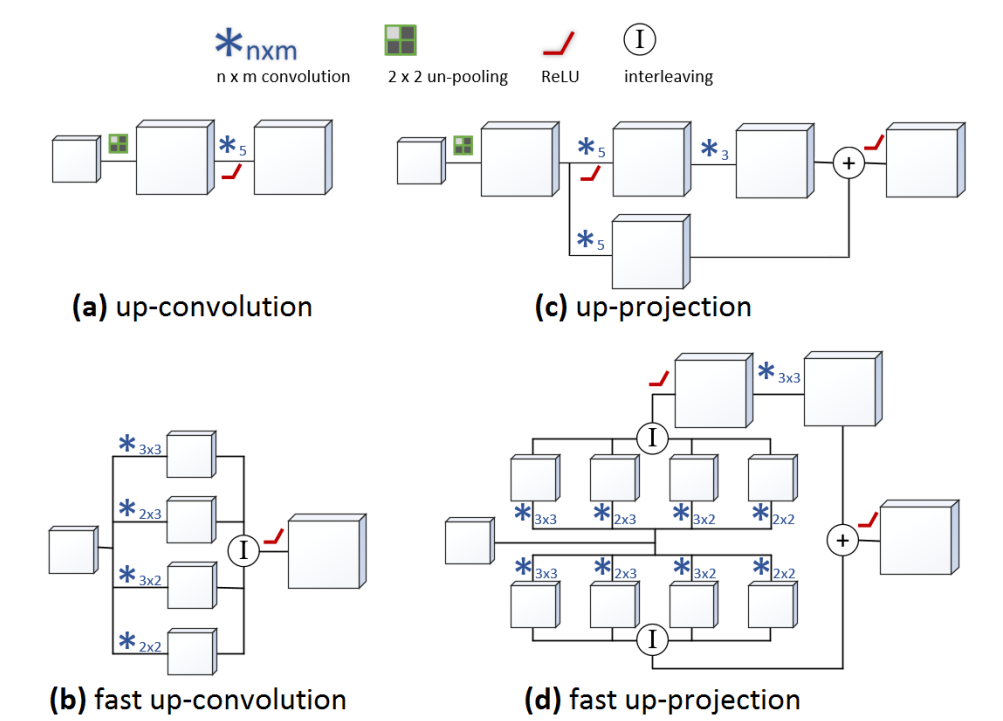
\includegraphics[scale=0.4]{figs/Laina}
\caption{Laina et al. \cite{Laina} up-sampling blocks inspired by ResNet blocks. To be read from left to right. They stack "Fast up-projection" blocks in their decoder. \label{fig:Laina}}
\end{figure}

% loss
For training their network they use the reverse Huber loss (berHu):
\begin{equation}
	\mathcal{B}(x) = 
	\begin{cases}
		|x| & \text{if } |x| \leq c \\
		\frac{x^{2} + c^{2}}{2c} & \text{if } |x| > c
	\end{cases}
\end{equation}
\[
	\mathcal{L}_{berHu} = \mathop{\text{mean}}_{(i, j) \in \mathbf{Z}^{*}} \mathcal{B}(\mathbf{Z}(i, j) - \mathbf{Z}^{*}(i, j))
\]
$\mathcal{B}$ is formulated in such a way that it is continuous and differentiable.
It behaves like an $l^{1}$ loss function in $[-c, c]$ and like an $l^{2}$ loss function outside that interval.
Laina et al. define $c$ batch-wise so that it is 20\% of the maximal per-batch error:
\[
	c = \frac{1}{5} \mathop{\text{max}}_{
		\substack{
			(\mathbf{Z}, \mathbf{Z}^{*}) \in \text{batch} \\
			(i, j) \in \mathbf{Z}^{*}
		}
	} \big| \mathbf{Z}(i, j) - \mathbf{Z}^{*}(i, j) \big|
\]
This is just an empirical heuristic they tuned, other choices for $c$ are also possible.
The authors motivate this loss function by noticing that depth values follow a heavy-tailed distribution (e.g. a log-normal distribution) and berHu loss is thus better suited considering that they work in linear-scale.
This could also explain \cite{Laina} why working in the log-scale was beneficial for Eigen et al., since the logarithm of a log-normal random variable follows a normal distribution which is in general well-behaved.

%%%%%%%%%%%%%%%%%%%%%%%%%%%%%%%%%%%%%%%%%
%                 DIW
%%%%%%%%%%%%%%%%%%%%%%%%%%%%%%%%%%%%%%%%%
\subsection{DIW}
Chen et al. \cite{DIW} tackle \textit{relative} depth estimation in the wild.
They both propose a method for training a model to learn relative depth and introduce a new dataset "Depth in the Wild" (\texttt{DIW}) which is discussed in the "Datasets" section.
The former is here treated.

First they consider an encoder-decoder architecture with long range skip connections as shown in figure \ref{fig:DIW_architecture}.
They take it from other authors and modify it using Inception blocks \cite{Inception}.

% architecture
\begin{figure}
\centering
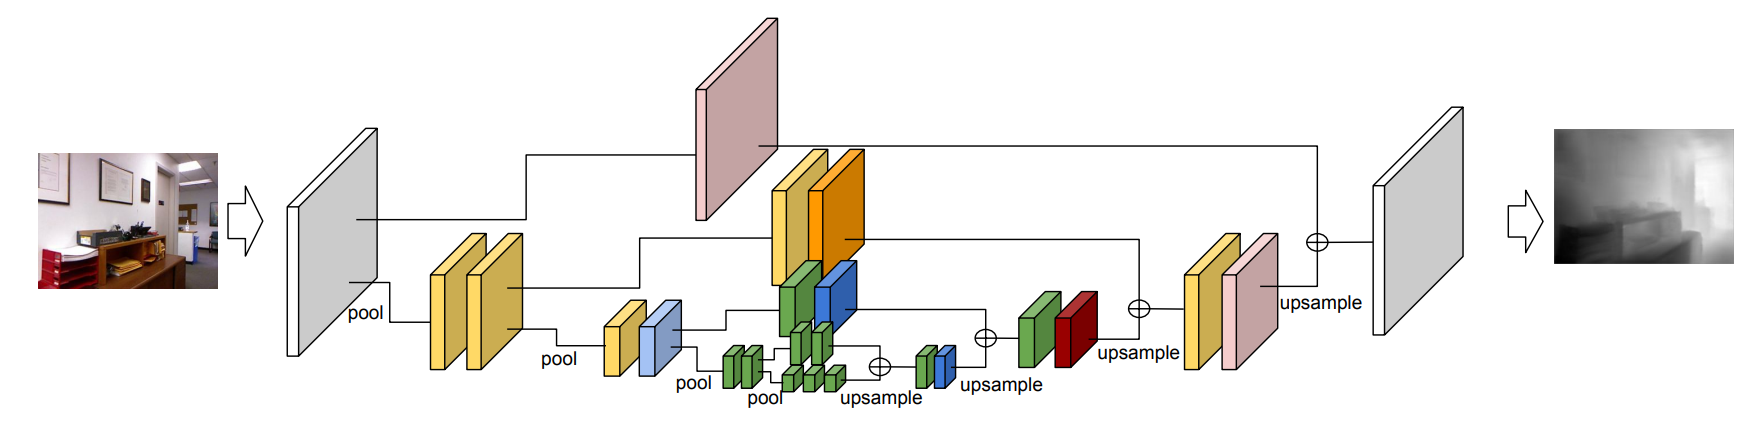
\includegraphics[scale=0.4]{figs/DIW_architecture}
\caption{Chen et al. \cite{DIW} architecture. \label{fig:DIW_architecture}}
\end{figure}

% comments
As they point out, their training method is not architecture-dependent and therefore other choices can be made.
The important thing is that their network outputs a depth map $\mathbf{Z}$ of its input image, this depth map is to be rather interpreted as \textit{relative}, meaning that it can be \textit{only} used for comparing depths between pairs of pixels.
For instance if $\mathbf{p_{1}}$ and $(k,l)$ are two pixels, $\mathbf{Z}(i, j) > \mathbf{Z}(k,l)$ implies that $\mathbf{Z}^{*}(i, j) > \mathbf{Z}^{*}(k,l)$.
Formally a relative depth map equals its metric depth map up to a pixel-wise monotonic transformation\footnote{For this reason, relative depth maps are not expressed in a specified scale, unlike metric depth map which can be expressed in linear-scale, log-scale, ...}.

% loss
For training such a network they employ a \textit{ranking loss} which encourages pairs of pixels to be ordered in a certain way.
Hence, they sample $K$ pairs of pixels from the ground-truth metric depth map and based on their relative depth adjust the predicted relative depth map in those locations:
\[
	\mathcal{L}_{ranking} = \mathop{\text{mean}}_{
		\substack{
			\text{sample } K \text{ pairs}\\
			 \mathbf{p}^{*}_{1} \neq \mathbf{p}^{*}_{2} \in \mathbf{Z}^{*}}
		}
	\begin{cases}
		\text{log} \, ( 1 + \text{exp} \, ( \mathbf{Z}(\mathbf{p}^{*}_{1}) - \mathbf{Z}(\mathbf{p}^{*}_{2}) )) &
			\text{if } \mathbf{Z}^{*}(\mathbf{p}^{*}_{1}) \ll \mathbf{Z}^{*}(\mathbf{p}^{*}_{2}) \\
		\text{log} \, ( 1 + \text{exp} \, ( \mathbf{Z}(\mathbf{p}^{*}_{2}) - \mathbf{Z}(\mathbf{p}^{*}_{1}) )) &
			\text{if } \mathbf{Z}^{*}(\mathbf{p}^{*}_{2}) \ll \mathbf{Z}^{*}(\mathbf{p}^{*}_{1}) \\
		(\mathbf{Z}(\mathbf{p}^{*}_{1}) - \mathbf{Z}(\mathbf{p}^{*}_{2}) )^{2} &
			\text{if } \mathbf{Z}^{*}(\mathbf{p}^{*}_{1}) \approx \mathbf{Z}^{*}(\mathbf{p}^{*}_{2})
	\end{cases}
\]
For deciding whether $\mathbf{Z}^{*}(\mathbf{p}^{*}_{1})$ and  $\mathbf{Z}^{*}(\mathbf{p}^{*}_{2})$ are $\ll$, $\gg$ or $\approx$ they use a dataset-dependent threshold $\tau$:

\begin{align*}
	\mathbf{Z}^{*}(\mathbf{p}^{*}_{1}) & \ll \mathbf{Z}^{*}(\mathbf{p}^{*}_{2}) \quad
		\text{if } \mathbf{Z}^{*}(\mathbf{p}^{*}_{1}) < \mathbf{Z}^{*}(\mathbf{p}^{*}_{2}) - \tau\\
	\mathbf{Z}^{*}(\mathbf{p}^{*}_{1}) & \gg \mathbf{Z}^{*}(\mathbf{p}^{*}_{2}) \quad
		\text{if } \mathbf{Z}^{*}(\mathbf{p}^{*}_{1}) > \mathbf{Z}^{*}(\mathbf{p}^{*}_{2}) + \tau\\
	\mathbf{Z}^{*}(\mathbf{p}^{*}_{1}) & \approx \mathbf{Z}^{*}(\mathbf{p}^{*}_{2}) \quad
		\text{if } |\mathbf{Z}^{*}(\mathbf{p}^{*}_{1}) - \mathbf{Z}^{*}(\mathbf{p}^{*}_{2})| \leq \tau
\end{align*}

It's very unlikely that two distinct pixels share the same identical depth value, thus the equality definition must be relaxed.

%%%%%%%%%%%%%%%%%%%%%%%%%%%%%%%%%%%%%%%%%
%                 ReDWeb
%%%%%%%%%%%%%%%%%%%%%%%%%%%%%%%%%%%%%%%%%
\subsection{ReDWeb}
Xian et al. \cite{ReDWeb} continue to study the problem of monocular relative depth estimation in the wild in the same way as Chen et al. \cite{DIW} did: they introduce a new dataset "Relative Depth from Web" (\texttt{ReDWeb}) and propose a training methodology.
The focus of this discussion is on the latter.
Contrary to \cite{DIW}, here the authors put more emphasis on the design of the architecture they use which is shown in figure \ref{fig:ReDWeb_architecture} below.

% architecture
\begin{figure}
\centering
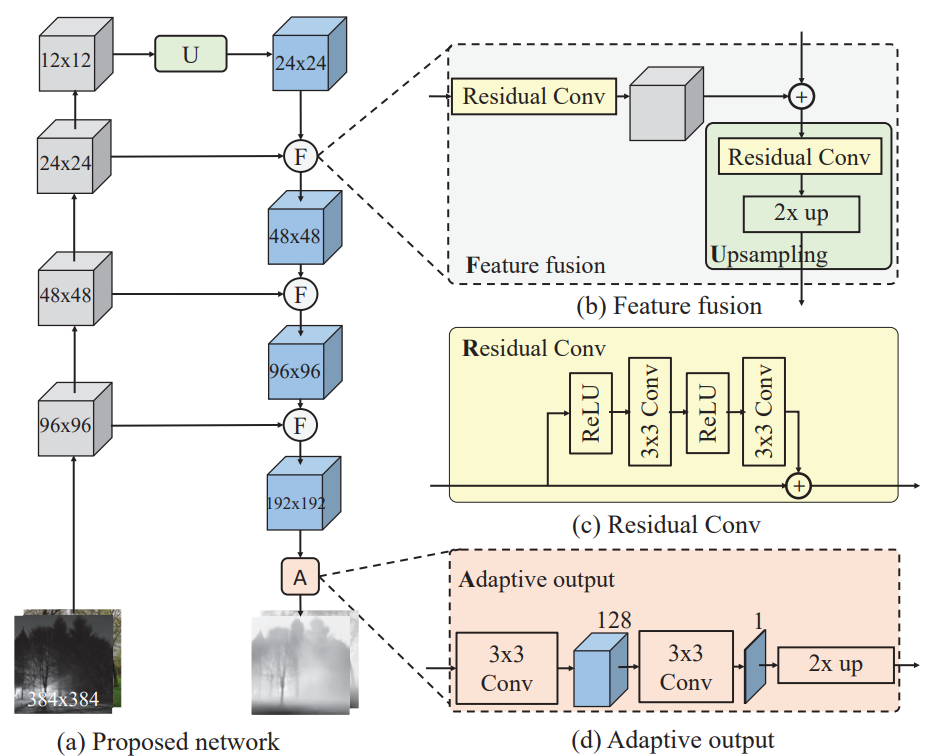
\includegraphics[scale=0.4]{figs/ReDWeb_architecture}
\caption{Xian et al. \cite{ReDWeb} architecture, the encoder backbone is based on ResNet \cite{ResNet} adding a multi-scale fusion module (b) connecting encoded feature maps with decoded ones. \label{fig:ReDWeb_architecture}}
\end{figure}

The idea of their training method is the same of Chen et al., the difference is in the choice of pixel pairs to analyze per image: in \cite{DIW} they were fixed per image, here instead are online sampled.
The sampling procedure produces imbalanced ordinal relations where the number of equal relation is far less than the other two relations.
The solution proposed by Xian et al. is to ignore the pixel pairs that result in the smallest loss and trim the 25\% of sampled pairs that less contribute to the loss function.
In this way two things are achieved: the ratio of the equal relation in the sampling increases and the network is enforced to focus on \textit{hard} pairs during training.

%%%%%%%%%%%%%%%%%%%%%%%%%%%%%%%%%%%%%%%%%
%               denseViT
%%%%%%%%%%%%%%%%%%%%%%%%%%%%%%%%%%%%%%%%%
\subsection{denseViT}
In \cite{denseViT} Ranftl et al. use the ViT \cite{ViT} architecture for monocular affine depth estimation following the MiDas training procedure \cite{MiDas}, their architecture is called Dense Prediction Transformer (DPT).
They substitute the usual fully convolutional encoder with ViT blocks, see figure \ref{fig:denseViT_architecture}.
The main idea is to process image patches using ViT modules and to re-assemble the obtained tokens as their respective patches creating a feature map.
In this way ViT blocks can be combined with usual techniques as convolutions and transposed convolutions for the decoding phase.
Ranftl et al. follow the usual U-Net \cite{UNet} scheme building an encoder-decoder architecture with information flowing from shallow layers of the encoder to deeper layers of the decoder.
The general architecture is represented in \ref{fig:denseViT_architecture}.
Thanks to the MiDas \cite{MiDas} training scheme and the very large meta-dataset (1.4 M images) \texttt{MIX 6} they introduced, DPT reaches and surpasses "state of the art" methods of the time.
Transformers have been known to better scale with dataset size than CNN based architectures do and Ranftl et al. work leverages on this fact \cite{ViT}.

% architecture
\begin{figure}
\centering
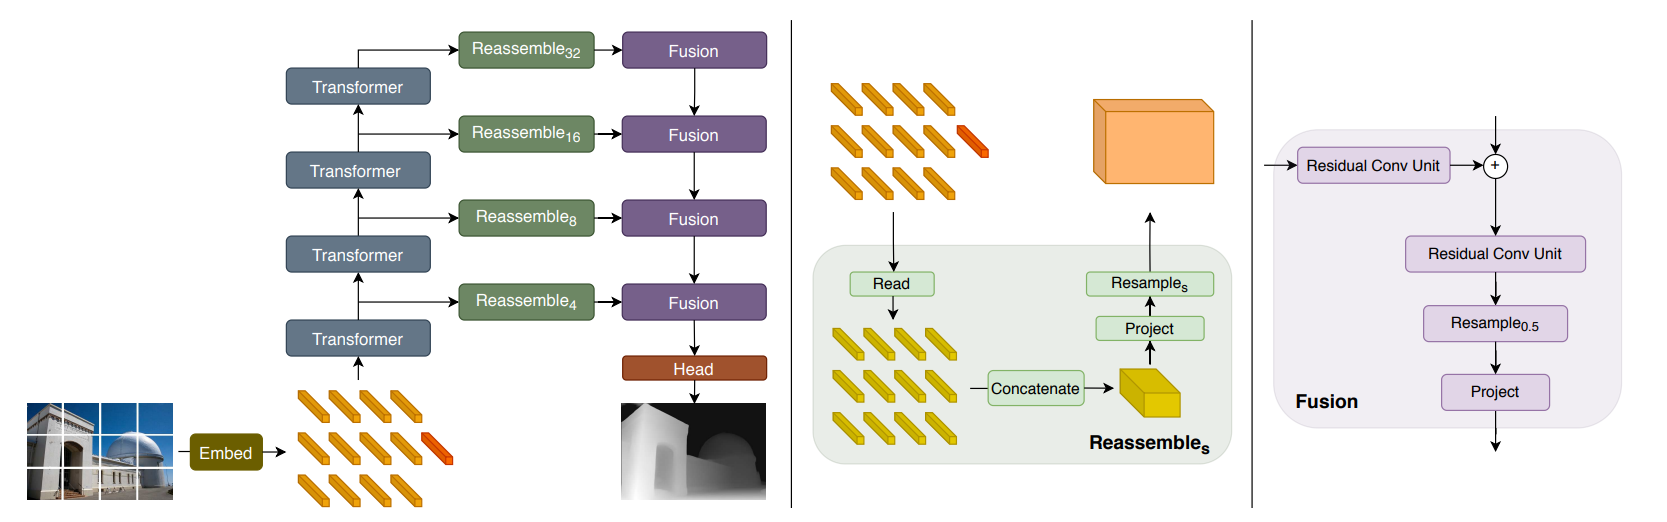
\includegraphics[scale=0.3]{figs/denseViT_architecture}
\caption{Ranftl et al. architecture \cite{denseViT}. \textit{Left}: the general architecture; \textit{Center}: how encoded tokens are processed to get a feature map; \textit{Right}: how multi-scale feature maps are fused during the decoding phase. \label{fig:denseViT_architecture}}
\end{figure}

%%%%%%%%%%%%%%%%%%%%%%%%%%%%%%%%%%%%%%%%%%%%%%%%%%%%%%%%%%%%%%%%%%%%%%%%
\section{Bin Methods}
\label{s:bin_methods}
Instead of regressing continuous depth values, these methods discretize the depth range and work with bins.
The discretization of depth range can be global and fixed \cite{depth_as_classification, ordinal_regression}, global but dependent on the image \cite{AdaBins}, local and dependent on the single pixel \cite{ZoeDepth}.
When probabilities (or scores, depending on the interpretation) are assigned to each bin, a depth value is actually computed which can eventually space in the whole range considered.
Find a summary in \ref{table:2}.

% summary table
\begin{center}
	\begin{table}
		\begin{tabular}{| c | c | c | c | c |}
		\hline
		\textbf{Year} & \textbf{Authors} & \textbf{Task} & \textbf{Formulation} & \textbf{Technique} \\
		\hline
		2018 &  Cao et al. \cite{depth_as_classification} & Metric DE & classification & CNN + CRF \\
		2018 & Fu et al. \cite{ordinal_regression} & Metric DE & ordinal regression & CNN \\
		2021 & Bhat et al. \cite{AdaBins} & Metric DE & hybrid regression & CNN + ViT\\
		2023 & Bhat et al. \cite{ZoeDepth} & Relative + Metric DE & hybrid regression & CNN + ViT\\
		\hline
		\end{tabular}
	\caption{Summary of treated bin methods for depth estimation. \label{table:2}}
	\end{table}
\end{center}

%%%%%%%%%%%%%%%%%%%%%%%%%%%%%%%%%%%%%%%%%
%        Depth as Classification
%%%%%%%%%%%%%%%%%%%%%%%%%%%%%%%%%%%%%%%%%
\subsection{Cao et al.}
Cao et al. \cite{depth_as_classification} formulate depth estimation as a pixel-wise classification task proposing a two-stage method.
Their idea is to discretize depth dividing its range into uniform bins.
The overall pipeline is illustrated in figure \ref{fig:depth_as_classification}

% architecture
\begin{figure}
	\centering
	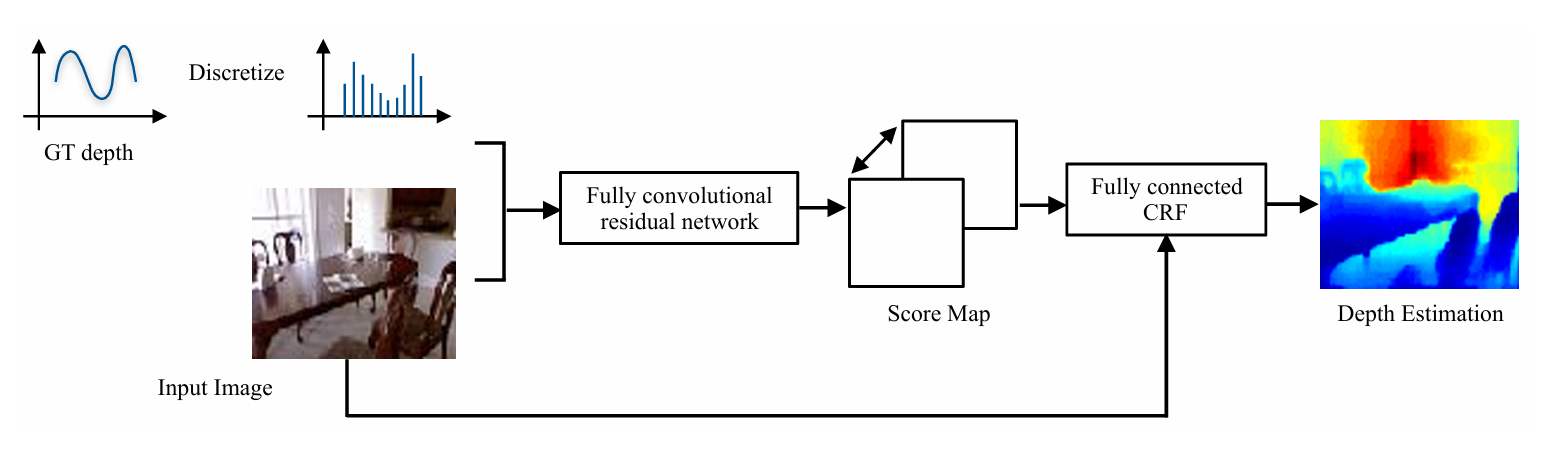
\includegraphics[scale=0.35]{figs/depth_classification}
	\caption{Cao et al. architecture \cite{depth_as_classification}. \label{fig:depth_as_classification}}
\end{figure}

% depth discretization
After an empirical investigation they decide to equally discretize the ground-truth \textit{log} depth range into $B$ bins.
Hence, assuming depth values range between $Z_{\text{min}}$ and $Z_{\text{max}}$, they consider $B+1$ points:
\[
	Z_{\text{min}}=Z_{0} < Z_{1} < Z_{2} < \dotsc < Z_{B} = Z_{\text{max}}
\]\[
	\text{such that} \quad \text{log} \, Z_{b+1} - \text{log} \, Z_{b} =
	\frac{\text{log} \, Z_{\text{max}} - \text{log} \, Z_{\text{min}}}{B}
	\quad b = 0, 1, \dotsc, B-1
\]

% prediction pipeline
The first stage of their method computes for each pixel the probability that its depth falls within a certain bin: if $\mathbf{Z}^{*}$ is the ground-truth depth map, for each pixel $(i, j) \in \mathbf{Z}^{*}$ they give an estimate of:
\[
	\mathbf{P}^{*}_{b}(i, j) = \mathbb{P} \, \{\mathbf{Z}^{*}(i, j) \text{ is between } Z_{b} \text{ and } Z_{b+1}\} \quad b = 0, 1, \dotsc, B-1
\]
This is achieved by a ResNet \cite{ResNet} backbone trained to output a probability map $\mathbf{P}$ of size $W \times H \times B$ with as many channels as bins and a resolution reduced by a factor of 8 w.r.t. the initial image $\mathbf{I}$ of size $W \times H \times 3$ taken as input.
This is then up-sampled by means of bilinear interpolation to the image size.
To obtain probability distributions, a softmax function is applied pixel-wise across prediction channels.

This estimated probability distribution map is converted into a label map:
\[
	\mathbf{L}(i, j) = \mathop{\text{arg max}}_{b \in \{ 0, \dotsc, B-1\}} \mathbf{P}_{b}(i, j)
\]

% loss
The loss employed is a variant of the multinomial logistic loss.
Assume ground-truth depth map $\mathbf{Z}^{*}$ is discretized to its label map $\mathbf{L}^{*}$:
\[
	\mathbf{L}^{*}(i, j) = b \text{ such that } \mathbf{Z}^{*}(i, j) \text{ is in the } b\text{-th bin}
\]
The loss can be expressed as:
\[
	\mathcal{L} =
		- \mathop{\text{mean}}_{(i, j) \in \mathbf{L}^{*}}
		\sum_{b = 0}^{B-1}
		e^{-(b - \mathbf{L}^{*}(i, j))^{2}}
		\text{log} \, \mathbf{P}_{b}(i, j)
\]
The factor $e^{-(b - \mathbf{L}^{*}(i, j))^{2}}$ makes the contribution of a predicted label proportional to its closeness to the ground truth label.
This is meaningful because labels are interpreted as discrete depth values.

% comments on post-processing
Cao et al. use a fully-connected Conditional Random Field (CRF) to post-process the predicted depth label map in the second stage.
Simply put, a CRF is a \textit{global} optimization procedure that adjusts discrete variables to minimize a certain quantity which encodes desired properties.
A fully-connected CRF is a special kind of CRF.
Not going into details, check \cite{computer_vision} for more.

The optimized label map $\mathbf{L}$ must be converted back to a depth map $\mathbf{Z}$.
The authors map labels to their respective bin centers by means of the following formulas:
\[
	\quad c_{b} = \frac{Z_{b} + Z_{b+1}}{2} \quad b = 0, 1, \dotsc, B-1
\]\[
	\mathbf{Z}(i, j) = c_{\mathbf{L}(i, j)}
\]
This sums up \cite{depth_as_classification}.

%%%%%%%%%%%%%%%%%%%%%%%%%%%%%%%%%%%%%%%%%
%        Ordinal Regression
%%%%%%%%%%%%%%%%%%%%%%%%%%%%%%%%%%%%%%%%%
\subsection{Fu et al.}
Fu et al. \cite{ordinal_regression} continue this line of research by adopting a slightly different approach which proved more effective.
They formulate depth estimation as an \textit{ordinal regression} problem.
The formal setting is very similar to the one of Cao et al., I will now illustrate the differences.
First, their method is end-to-end as shown in the image \ref{fig:Fu_ordinal}.

% architecture
\begin{figure}
	\centering
	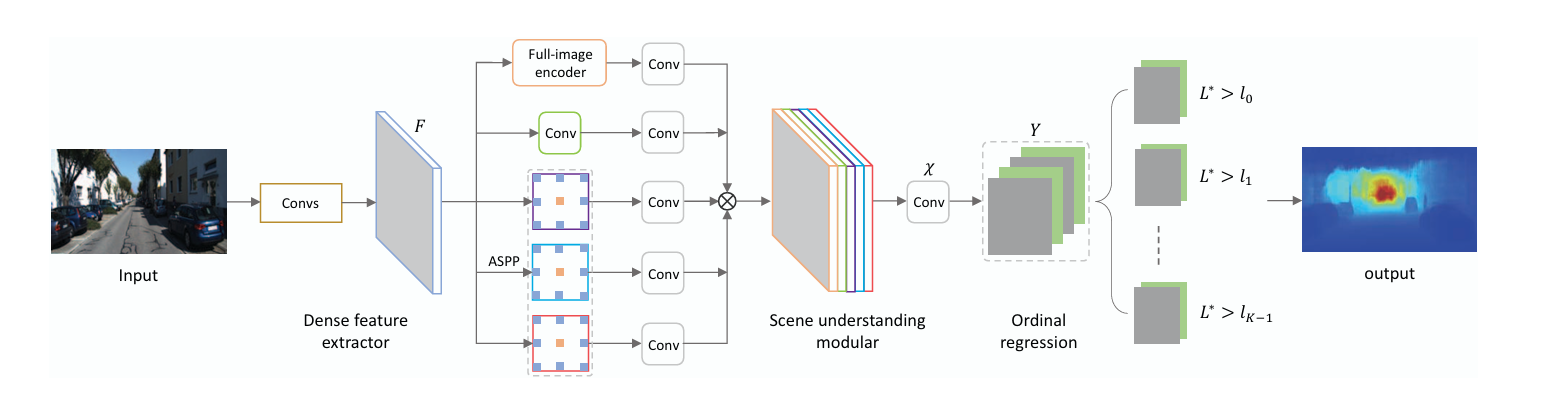
\includegraphics[scale=0.35]{figs/Fu_ordinal}
	\caption{Fu et al. architecture \cite{ordinal_regression}. It employs an "atrous spatial pyramid pooling" module (ASPP) which deals with multiscale details by working with various dilation rates for convolutions. \label{fig:Fu_ordinal}}
\end{figure}

Second, a more sophisticated architecture estimates $\mathbf{P}^{*}$ from $\mathbf{I}$, and it is composed of different modules, some working in parallel and some in serial.
They use dilated convolutions for enlarging the field of view without decreasing spatial resolution or increasing number of parameters \cite{ordinal_regression} and $1 \times 1$ convolutions for cross-channel interactions \cite{ordinal_regression}.
Third, they interpret $\mathbf{P}^{*}_{b}(i, j)$ as $\mathbb{P} \, \{ \mathbf{Z}^{*}(i, j) < Z_{b+1} \}$, namely the probability that the pixel $(i, j)$ corresponds to a point that doesn't fall farther than the $b$-th depth bin.
If a pixel $(i, j)$ corresponds to bin $\mathbf{L}^{*}(i, j)$ then $\mathbf{P}_{b}(i, j)$ must be maximized for $b \leq \mathbf{L}^{*}(i, j)$ and minimized for $b > \mathbf{L}^{*}(i, j)$, hence the following loss function:
\[
	\mathcal{L} = - \mathop{\text{mean}}_{(i, j) \in \mathbf{L}^{*}}
	\left(
		\sum_{b=0}^{\mathbf{L}^{*}(i, j)} \text{log} \,( \mathbf{P}_{b}(i, j)) \quad +
		\sum_{b=\mathbf{L}^{*}(i, j) + 1}^{B-1} \text{log} \, (1 - \mathbf{P}_{b}(i, j))
	\right)
\]
The predicted label map $\mathbf{L}$ is defined as:
\[
	\mathbf{L}(i, j) = | \{b \, \text{ such that } \, \mathbf{P}_{b}(i, j) > 0.5\} |
\]
Ideally $\mathbf{P}_{b}(i, j) > 0.5$ for $b \leq \mathbf{L}^{*}(i, j)$ and $\mathbf{P}_{b}(i, j) \leq 0.5$ for $b > \mathbf{L}^{*}(i, j)$, so that $\mathbf{L}(i, j) = \mathbf{L}^{*}(i, j)$.
In case $\mathbf{P}_{b}(i, j)$ is above $0.5$ for every $b$, $(i, j)$ can be considered at a depth outside the range $Z_{\text{min}}$, $Z_{\text{max}}$, e.g. it can correspond to a point at $\infty$ depth like the sky.

%%%%%%%%%%%%%%%%%%%%%%%%%%%%%%%%%%%%%%%%%
%               AdaBins
%%%%%%%%%%%%%%%%%%%%%%%%%%%%%%%%%%%%%%%%%
\subsection{AdaBins, LocalBins and ZoeDepth}
Shariq Farooq Bhat and other researchers worked a lot on single image depth estimation using bin-methods and developed three important works: AdaBins \cite{AdaBins}, LocalBins \cite{LocalBins} and ZoeDepth \cite{ZoeDepth}.

\paragraph{AdaBins} In the first work, Bhat et al. \cite{AdaBins} generalize the ideas from Fu et al. \cite{ordinal_regression}.
They observe that depth distribution vary to a large extent between different scenes, therefore depth bins must be adapted per image.
The pipeline is illustrated in figure \ref{fig:adabins}.

% architecture
\begin{figure}
	\centering
	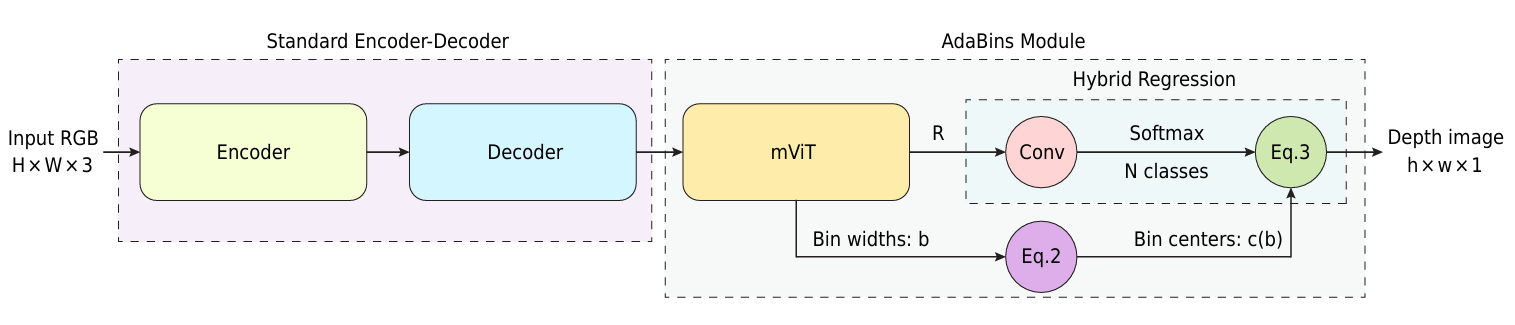
\includegraphics[scale=0.35]{figs/adabins}
	\caption{Bhat et al. architecture \cite{AdaBins}. \label{fig:adabins}}
\end{figure}

The image $\mathbf{I}$ is processed by an encoder $\mathcal{E}$ decoder $\mathcal{D}$ architecture to obtain what the authors call \textit{decoded features}, that is a multichannel feature map $\mathbf{F}$:
\[
	\mathbf{F} = \mathcal{D}(\mathcal{E}(\mathbf{I})) \quad H \times W \times C \text{ feature map}
\]
The rest of the pipeline is the "AdaBins" block, as the authors call it.
The idea of Bhat et al. for estimating the bins adaptively is to extract \textit{global} information and to use that for the purpose.
A Vision Transformer (ViT) \cite{ViT} is used for exploiting global context.
A Vit takes an image as input, divide it into grid patches, process them favouring information exchange and outputs a vector for each of them. Calling the Vit $\mathcal{T}$, the image is divided into $S$ patches:
\[
	\mathcal{T}: \mathbb{R}^{H \times W \times C} \rightarrow \mathbb{R}^{S \times C}
\]
Hence $\mathcal{T}(\mathbf{F}) = (\mathcal{T}(\mathbf{F})_{1}, \dotsc, \mathcal{T}(\mathbf{F})_{S})$ are $S$ vectors of $\mathbb{R}^{C}$.
Each of these vectors encodes global information, any one of them can be used to get the bins, e.g. the first one $\mathcal{T}(\mathbf{F})_{1}$.
The authors construct the discretization of the depth range by computing relative bin-widths from global information:
\[
	(w_{0}, \dotsc, w_{B-1}) = \text{learnable mapping }(\mathcal{T}(\mathbf{F})_{1})
\]\[
	\text{such that } \forall b \,\, w_{b} > 0 \, \text{ and } \, \sum_{b=0}^{B-1} w_{b} = 1
\]
Bins extrema $Z_{b}$ and bin centers $c_{b}$ can be calculated knowing the depth range $Z_{\text{max}}$, $Z_{\text{min}}$ (dataset dependent) and by using the following formula:
\[
	w_{b} = \frac{Z_{b+1} - Z_{b}}{Z_{\text{max}} - Z_{\text{min}}} \quad b=0, 1, \dotsc, B-1
\]
Now that the depth range has been discretized, labels probabilities need to be computed.
For this final step global information is exploited again: $\mathbf{F}$ (which has $C$ channels) is convolved with each $\mathcal{T}(\mathbf{F})_{s}$ $s=1,\dotsc,S$, which are thought as $C \times 1 \times 1$ kernels and an $H \times W \times S$ map is returned which is in turn pixel-wise processed to obtain a probability map $\mathbf{P}$ of size $H \times W \times B$.

Finally, depth can be estimated.
To avoid discretization artifacts they compute the depth as the following linear combination:
\[
	\mathbf{Z}(i, j) = \sum_{b=0}^{B-1} c_{b} \, \mathbf{P}_{b}(i, j)
\]
Therefore, in this work, $\mathbf{P}_{b}(i, j)$ can be interpreted as an approximation to the p.d.f. of the pixel-wise depth distribution.

While for optimizing the depth map obtained Bhat et al. use a Scale-Invariant loss \cite{Eigen}, for optimizing the bin centers $c_{b}$ they adopt the following:
\[
	\mathcal{L}_{\text{bins}} =
	\sum_{(i, j) \in \mathbf{Z}^{*}} \mathop{\text{min}}_{b \in \{0, \dotsc, B-1\}} \, (\mathbf{Z}^{*}(i, j) - c_{b})^{2} \quad+
	\sum_{b \in \{0, \dotsc, B-1\}} \mathop{\text{min}}_{(i, j) \in \mathbf{Z}^{*}} \, (\mathbf{Z}^{*}(i, j) - c_{b})^{2}
\]
This loss, called "bidirectional Chamfer Loss" \cite{AdaBins}, encourages the bin center distribution to match the ground-truth depth distribution.

%%%%%%%%%%%%%%%%%%%%%%%%%%%%%%%%%%%%%%%%%
%              LocalBins
%%%%%%%%%%%%%%%%%%%%%%%%%%%%%%%%%%%%%%%%%

\paragraph{LocalBins} In \cite{LocalBins} Bhat et al. notice that depth discretization must be performed locally, pixel-wise, rather than globally.
In fact, depth values distributions can widely vary across a single image.
The overall procedure is shown in figure \ref{fig:localbins}.

% architecture
\begin{figure}
	\centering
	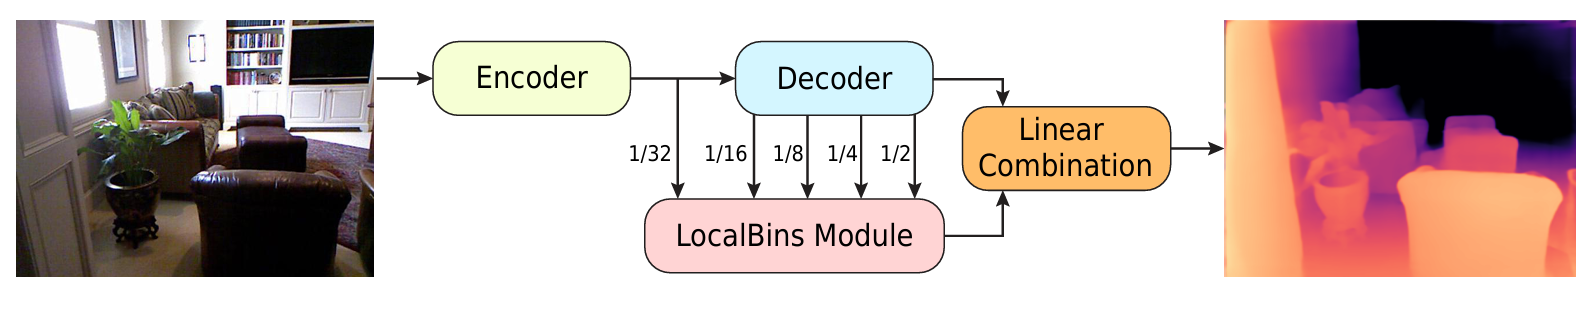
\includegraphics[scale=0.3]{figs/localbins}
	\caption{Bhat et al. architecture \cite{LocalBins}. LocalBins module contains pixel-wise operations and estimate local neighborhood bin density for each pixel location. \label{fig:localbins}}
\end{figure}

Instead of directly predicting the whole depth range discretization, Bhat et al. employ a coarse-to-fine binning strategy.
They start from $B_{\text{seed}}$ bins and during the decoding phase, exploiting multi-scale processing, they apply a bin-splitter module that doubles the number of bins.
Bins are specified through their widths, like in AdaBins, but pixel-wise, so a map $\mathbf{W} \in \mathbb{R}^{H \times W \times B}$ is computed at each step of the decoding phase with $B$ doubling each time.
To "split the bins" the idea is to divide each bin-width into two more by means of a convex combination.
Basically a map $\mathbf{A}$ of same shape as $\mathbf{W}$ is computed but with values in $(0, 1)$ and the new bin-widths are obtained by concatenating the two following tensors:
\[
	\mathbf{B}_{0} = \mathbf{A} \odot \mathbf{W}
\]\[
	\mathbf{B}_{1} = (1 - \mathbf{A}) \odot \mathbf{W}
\]\[
	\mathbf{B}_{\text{new}} = \text{concat} (\mathbf{B}_{0}, \mathbf{B}_{1})
\]
The training loss is similar to the Chamfer loss introduced above, but adapted to the multi-scale setting.
For further details see \cite{LocalBins}.

%%%%%%%%%%%%%%%%%%%%%%%%%%%%%%%%%%%%%%%%%
%              ZoeDepth
%%%%%%%%%%%%%%%%%%%%%%%%%%%%%%%%%%%%%%%%%
\paragraph{ZoeDepth} Eventually, Bhat et al. \cite{ZoeDepth} refine their ideas for computing depth bins pixel-wise in their work called "ZoeDepth".
The result is a two-stage method for estimating both relative and metric depth, the overall architecture is shown in figure \ref{fig:zoe_depth}.

% architecture
\begin{figure}
	\centering
	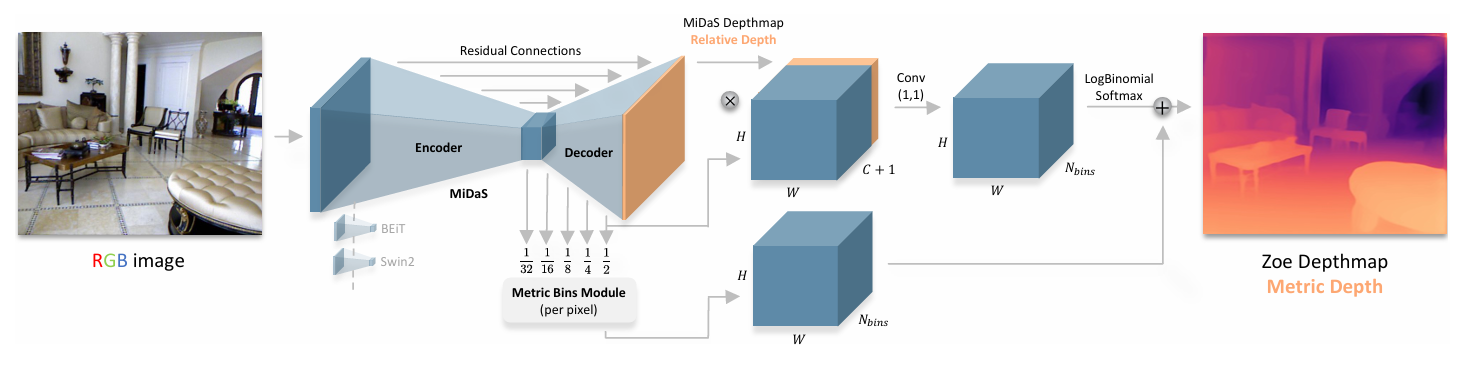
\includegraphics[scale=0.3]{figs/zoe_depth}
	\caption{Bhat et al. architecture \cite{ZoeDepth}. \label{fig:zoe_depth}}
\end{figure}

They use the multi-dataset training procedure of \cite{MiDas} and the general encoder-decoder architecture for estimating relative depth maps is taken from \cite{denseViT}.
To the decoder they attach a head, which they call "Metric Bins Module", for converting relative depth maps into metric depth maps.
Therefore, when training on relative depth datasets only the decoder output is used, whilst when training on metric depth datasets the output of the head is considered.
The Metric Bins Module works at multiple scales: given the lowest scale relative depth map returned by the decoder, a point-wise convolution estimates $B$ bin centers $\{\mathbf{C}_{0}, \mathbf{C}_{1}, \dotsc, \mathbf{C}_{B-1}\} \subset \mathbb{R}^{H \times W \times B}$ pixel-wise, then at successive finer scales other point-wise convolutions return $K$ "attractors" $\{\mathbf{A}_{1}, \mathbf{A}_{2}, \dotsc, \mathbf{A}_{K}\} \subset \mathbb{R}^{H \times W \times K}$, which serve the purpose to modify the previously computed bin distributions pixel-wise by computing an adjustment $\triangle \mathbf{C}_{b}$ for each bin center:
\[
	\triangle \mathbf{C}_{b} = \sum_{k=1}^{K} \frac{\mathbf{A}_{k} - \mathbf{C}_{b}}{1 + \alpha | \mathbf{A}_{k} - \mathbf{C}_{b} |^{\gamma}}
\]
Like before, they assign to each bin (pixel-wise) a probability $\mathbf{P}_{b}$ so that the predicted depth map is:
\[
	\mathbf{Z} = \sum_{i=0}^{B-1} \mathbf{C}_{b} \, \mathbf{P}_{b}
\]
In this formula bins are ordered since their ordering is not preserved during training depending on how the attractors influence.
To make sure not to obtain a difficult to interpret multi-modal probability distributions, the authors build $\mathbf{P}$ pixel-wise and across the bins-channel using the binomial distribution.
Hence, instead of predicting the actual probability values, binomial distribution parameters are computed.
To make things numerically stable they employ some more trickery I won't report.